\documentclass[table,a4paper,oneside]{book}

\usepackage{graphicx} % Allows insert of graphics
\usepackage{longtable} % Allows for multipage spanning tables
\usepackage{pdfpages} % Simplifies insertion of multipage PDF’s
\usepackage{natbib} % Puts in bibliography style
\usepackage[pdfborder=0 0 0]{hyperref} % Adds PDF links
\usepackage{mathptm} % Changes font
\usepackage{fancyhdr} % Allows the use of the fancy Header package
\usepackage{url} % Makes URL’s appear nicer and follow formatting rules
\usepackage{algorithm} % Allows Algorithmic insertions to be floated
\usepackage{algorithmic} % Allows Algorithms and Pseudocode
\usepackage{textcomp} % LaTeX support for the Text Companion fonts.
\usepackage{setspace} % Allows the use of the set space command
\usepackage{listings} % Allows the use of source code
\usepackage{colortbl} % Adds colour to rows etc
\usepackage{acronym} % Allows the use of acronyms in code - deals with printing acronyms out nicely
\usepackage{booktabs} % Allows the use of professional looking tables
\usepackage[a4paper,vmargin={25.4mm,25.4mm},hmargin={35.0mm,25.4mm}]{geometry} % Allows the changing of page borders

\setlength{\parindent}{0.0in} % Sets paragraph indentation to 0
\pagestyle{fancy}
\bibpunct{(}{)}{,}{a}{,}{,} % Defining the citation style
\newcommand{\degree}{\ensuremath{^\circ}} % Sets new command - Inserts degree symbol
\newcommand{\HRule}{\rule{\linewidth}{0.5mm}} % Set new command - Add blank line
\newcommand{\mtwo}{m\textsuperscript{2} } % Sets the command - Adds m^2.

% Acronym Definition
% \acrodef{label}[acronym]{written out form}
% \acrodef{acronym}{written our form}
\acrodef{ADB}{Approved Document B}
\acrodef{BCIS}{Building Cost Information Service}
\acrodef{CLG}{Department of Communities and Local Government}
\acrodef{CSV}{Comma Separated Value}
\acrodef{FPA}{Fire Protection Association}
\acrodef{FRS}{Fire and Rescue Service}
\acrodef{IRS}{Incident Reporting System}
\acrodef{IRMP}{Integrated Risk Management Plan}
\acrodef{RIBA}{Royal Institute of British Architects}

\begin{document}
\onehalfspacing
% Above command sets document to 1.5 line spacing
% Remove all above when creating thesis from Master document

\chapter{Methodology}
\label{chapter:Methodology}
\acresetall

\section{Literature Review}
\label{sec:Literature Review}
The initial step of the research was to identify a gap in the research. This was done by extensive reading into the subject area. Initially, from experience, there seemed to be a research gap into the cost effectiveness of passive protection. This was gathered from experience within the fire engineering design industry so further work was required to identify whether or not this was the case within the academic community. Reading was undertaken, focusing mainly on the fire based journals such as The Journal of Fire Protection, Fire Technology and the Fire Safety Journal. After these, the scope of the reading was extended to civil engineering articles and research referenced by previous papers. From this reading, it was confirmed that there was a lack of research about passive fire protection methods and costs. However, various papers such as Moeller's report about protection in Denmark \citep{KristianMoeller2001}, suggest that this is due to a lack of data and though, for many years, researchers have been suggesting that there exists an optimum combination of passive and active fire protections measures \citep{Baldwin1974, Corporation1991, Haack2004}. However, research and data collection on passive protection hasn't been a major focus and these studies recommended that more data was collected on passive protection measures.
\\
\\
Fire incident data for the UK was acquired from the \ac{CLG} and this was investigated. On analysis, it was found that data on passive fire protection was either not included on the original FDR 1 form and therefore not recorded. These fire incident records were taken from FDR 1 forms filled in by firefighters attending the scene of the incident and often the forms are incomplete or incorrect data is entered. Further data was collected from the Fire Protection Association (FPA) and this data, whilst appearing more complete and more accurately filled in (potentially as its source is from loss adjusters attending a fire incident, post cleanup and insurers being more concerned with accuracy and costs than firefighters might be at the time of recording), also failed to detail any passive fire protection measurements that could be used in analysis. Therefore, further pursuit of this avenue of research would be prove inconclusive as the data was not available to provide an evidence base and inform decisions.
\\
\\
However from reading and from previous experience, it was apparent that fire engineers in the UK only built buildings to specifications within the Building Regulations. Life safety requirements within the codes were met but no consideration was given for the building structure itself in a fire incident. Previous research by Ramachandran had investigated the cost benefits of installing extra protection measures into a building at the design stage \citep{Ramachandran1998} but little change appeared to have filtered through to the industry. In reading on the subject, Ramachandran mentions the calculations that can be used in a cost benefit tool but nothing is mentioned more is mentioned on the construction of a cost benefit tool.Yet, a report published in New Zealand \citep{Page2005} states as a recommendation that cost benefit tools should be constructed to help designers consider property protection within the design so that sustainable design can be achieved (through less fires and therefore reduced need for rebuilding). No other data could be found that suggested that this recommendation had been taken on board and the aim achieved. Therefore it was considered that one of the main outcomes of this research should be a methodology for a cost benefit tool.
\\
\\
Fire engineering is an costly procedure and is not undertaken lightly. The reason a fire engineer is employed is to save money on buildings where the architect wishes to cut costs in relation to fire safety measures specified in building codes. The building codes are restrictive and force the architect to make sacrifices in terms of aesthetics and other features. With the help of a fire engineer, a different method of meeting the regulations can be engineered and thus allowing the architect more freedom. This cost and effort means that the type of projects fire engineering designs are used in are larger, non residential projects. This is because it is far easier to construct houses to meet the building regulations through the use of \ac{ADB} \citep{Communities2006}. As such, fire engineering is not widely, if at all used in residential buildings and therefore, residential buildings were not considered as part of this project. In rare cases, large individual houses or large tower blocks containing a mixture of commercial and residential may have fire engineering used in the design and construction but it was not viewed that these were widespread to consider residential as part of this research.

\subsection{FDR 1 Incident Records}
\label{sec:FDR 1 Incident Records}
The FDR 1 data was provided by \ac{CLG} and is the result of filling in (paper) FDR 1 forms by the fire brigade at every fire incident attended. The data covered by the given dataset dates from 1998 until 2008, where it was replaced by the new, computerised \ac{IRS}. These records were collected by each individual \ac{FRS} and were stored locally until sent to \ac{CLG} who would then computerise the results.
\\
\\
The dataset does not contain all the FDR 1 records. When collated by the Government statisticians, not all the data was entered. A sampling system meant that only some data was inserted into the electronic database kept by \ac{CLG}. This sampling varied year by year. All incidents that contained a fatality or injury to an occupant or fire fighter was kept and then the rest of incidents were then sampled and entered into the database. Table \ref{tab:Sampling_Rates} shows the sampling rates used in the FDR 1 data set over the past decade. This was confirmed in an email from Jon Gamble (the head data analyst at the Fire Statistics Unit) in September 2010.

\begin{table}[htbp]
	\begin{center}
	\begin{tabular}{lr}
		\toprule
		\textbf{Year}	& \textbf{Sampling (\%)} \\
		\midrule
		1994	&	10 \\
		1995	&	40 \\
		1996 - 2004	&	20 \\
		2005	&	100 \\
		2006 - 2008	&	20 \\
		\bottomrule
	\end{tabular}
	\end{center}
\caption{FDR 1 Sampling Rates}
\label{tab:Sampling_Rates}
\end{table}

This sampling method would allow an estimate of the full results to be calculated, however, a weighting factor is also applied to the results. This weight value is the aggregate weighted value of the total number of fires in the \ac{FRS} area.
\\
\\
As the values of the weighting are unclear in exactly how they were obtained, it is assumed that the weighting value represents how many cases that meet the same criteria were in the sample. However, even with discussion with CLG statisticians, this point remained unclear and the decision was made to make calculations \textbf{only based on 2005 data} due to the fact the data for 2005 is represented in complete fullness (no samples were taken, all data was entered into the FDR 1 database and all weighting values are 1).
\\
\\
This decision does mean that the number of incidents available to investigate is lowered, however the incidents can be analysed, confident that the results are as accurate as entered by the original FRS as no further errors have been introduced by sampling errors. Yet it should still be considered that data errors could be possible from the original entry by the attending \ac{FRS}. However, there is currently no data on the potential accuracy of the inputted data and in this research, it will be taken as accurate, unless a result contradicts itself. This is due to the fact that this is the only large dataset of it's kind in the UK and no alternatives are available. Should a more accurate database be kept, then the methodology behind the analysis of this data should allow for more accurate results from more accurate data.
\\
\\
The initial database contained 978,944 records of fire incidents. However, this included data on buildings that weren't part of this study. This study focussed only on commercial, public and heritage buildings. After filtering by TOP code (the code defining the use of a building - listed in the FDR 1 Codelist \citep{HomeOfficeResearchDevelopment&StatisticsDirectorate1998}), there were a total of 191,311 records.

%TC:ignore
% Sets Texcount to Ignore
\begin{algorithm}
	\caption{Code to Filter FDR 1 data}
	\label{alg:Filtering_Code}
\begin{lstlisting}
sed -n 1p Lboro_9908.csv > Filtered_Buildings.csv
 awk -F , "$14=="X" {print}" Lboro_9908.csv >> Filtered_Buildings.csv
 awk -F , "$14=="Y" {print}" Lboro_9908.csv >> Filtered_Buildings.csv
 awk -F , "$14=="Z" {print}" Lboro_9908.csv >> Filtered_Buildings.csv
 \end{lstlisting}
\end{algorithm}
%TC:endignore
% Ends Texcount to Ignore

The data was filtered according the code in Algorithm \ref{alg:Filtering_Code}. This batch file used the command sed which copied the first line of the Lboro\_9908.csv file into the new filtered file as this first line contained the column heading and then used the awk command to search the 14\textsuperscript{th} column which contains the TOP code for the variable X which corresponds to the TOP code being searched for. This then prints the data into a new file called Filtered\_Buildings.csv. The command is repeated with Y and then Z and so on until all TOP units in question have been filtered out into the new file. The full code can be seen in the Appendix on page \pageref{code:FDR1_Data}. The  TOP codes that were filtered into Filtered\_Buildings.csv are shown in Table \ref{tab:TOP_Codes}. This gave a file that only contained records that were considered for further data analysis. From henceforth, when referring to the FDR 1 data, it is to be assumed that it is this Filtered Buildings dataset that is being referred to, unless otherwise stated.

\subsection{Fire Protection Association Data}
\label{sec:Fire Protection Association Data}
The \ac{FPA} data is a collection of fire incident records, collected by loss adjustors visiting sites of fires and submitted to an insurance company. This is then submitted to the \acl{FPA} for collating and statistical use, however only the records of all fires over \pounds 100,000 or an instance where someone was killed are sent to the \ac{FPA} for collating. This means that the data collected by the \ac{FPA} focuses on the large loss claims in the UK. As might be expected from the large costs, this database mainly consists of commercial, public and heritage data, though it does include some instances of residential properties which will be later stripped out.
\\
\\
The data made available for this project was provided ``as is'', meaning that a live snapshot was taken of the database (as it is continually being updated) and made available for analysis. The only changes to the data was the removal of all information that could have potentially identified an insurer, an incident or a claimant. Data was not sampled or changed in anyway and the data was provided as a raw data dump. This meant analysis could be performed on the records with less pre-processing.
\\
\\
In comparison to the FDR 1 data, the \ac{FPA} database is much smaller. Initially the dataset contained 963 records of incidents. On analysing the data further, it was found that the database contained both data on fire and explosions - these were in the database as the source of the incident. As such, any records where the cause was considered to be an explosion were removed from the dataset using the PASW SPSS Statistics software. The cause of the incident was not mutually exclusive in the database and therefore some records were recorded as having started by fire and also an explosion. As the research is only focussing on fires and in the authors view, an incident is either started by a fire and progresses to an explosion or the incident is started by an explosion and a fire ensues, these incidents were also removed from the dataset. As described in the \nameref{sec:FDR 1 Incident Records} section on page \pageref{sec:FDR 1 Incident Records} , the research focuses on commercial, public and heritage buildings and does not include residential occupancies. As such, the records in the \ac{FPA} dataset that occurred in residential occupancies are removed. This pre-processing allowed the dataset to be saved without having to remove the irrelevant incidents before each stage of analysis. Once saved in PASW SPSS, the dataset was also saved as a \ac{CSV} file to allow it to used in other programs alongside SPSS.
\\
\\
Unlike the FDR 1 data, the \ac{FPA} data contains cost estimates for each incident. This will allow cost estimates of damage to be considered in the analysis section. These cost figures are estimates, based on the loss adjustors experience and judgement. This means that the data submitted by each loss adjustor is likely to differ in the cost estimates. However, as the database continues to grow and get updated and individual cases approach the conclusion, the actual cost of fires will be submitted into the database and thus would give more accurate results. In the mean time, the estimates currently in the database are the best method of estimating the costs of a fire. The \ac{FPA} have no information on how these estimates are calculated. The methods are left upto the individual insurance companies and loss adjustors.

\subsection{BCIS Data}
\label{sec:BCIS Data}
The \ac{BCIS} is a commercial service that records the cost of new and modification costs for building design. It's database and tools are designed to allow the construction industry to accurately estimate prices of a new tender.
\\
\\
The data is collected from construction firms after construction is complete and is split into various figures, the most important one for this research being the cost per \mtwo. The data within the database is split quite extensively into different categories under building occupancies. For example see Table \ref{tab:BCIS_School_Data}, taken from the BCIS tool which shows the sort of detail the database can go into.

\begin{table}[htbp]
	\begin{center}
	\begin{tabular}{ll}
		\toprule
		\textbf{BCIS Reference Number}	& \textbf{Category} \\
		\midrule
		710	&Schools	\\
		711	&Nursery schools/creches	\\
		712	&Primary schools	\\
		712.1	&Middle schools	\\
		712.12	&Primary/middle schools - specialised teaching blocks \\
		712.8	&Primary Schools - mixed facilities \\
		713	&Secondary schools (high schools)	\\
		713.1	&Secondary schools - specialised teaching blocks \\
		713.8	&Secondary Schools - mixed facilities \\
		714	&Sixth form/tertiary colleges	\\
		714.1	&Sixth form specialised teaching blocks \\
		714.8	&Sixth form - mixed facilities	\\
		\bottomrule
	\end{tabular}
	\end{center}
\caption{School Data from BCIS Database}
\label{tab:BCIS_School_Data}
\end{table}

As can be seen, this splitting of data does allow very precise measurements if needed for specific uses, however, splitting the data across these categories mean that some of the buildings do not have enough costs associated with them to make it possible to statistically analyse them or rely on the data they provide. For example, some categories have only 1 data entry and therefore the average is the cost of that single project. To be used in later analysis, it was combined with the data from the \ac{FPA}.
\\
\\
It should be noted that, ideally, a subscription to BCIS would be needed to update the values in the proposed fire safety tool as the values are only available to BCIS members. Therefore to get the most up to data costs, a subscription to the service would be required. Using this dataset alongside other, such as the values in the \ac{FPA} dataset can provide a validation step.

\subsection{Rateable Values}
\label{sec:Rateable Values}

Initially the rateable value of a building was considered as a method of estimating costs for a fire. The rateable value for a property is a measure of it's rental value and is collected by the Valuation Office Agency and is updated every few years. This value, if used in a calculation for the the cost of a fire however, would grossly underestimate the costs of a fire because this rateable value only covers the cost of the rent of the property – no measure of the internal fittings and fixtures is taken into account. It is split into the different building occupancies and also is searchable by location within the UK regions (i.e. South West, London, East Midlands, West Midlands). This would allow the use of location aware pricing structures to be placed within the tool but because of the limitation of the data, it should not be used for the purpose. However, it can prove useful as a baseline value when compared with the results from another cost calculation – if the value of the alternative calculation is below the value of the ratable value, then that result can be investigated closely as to why it's smaller than this value. This will add a layer of validation to the tool itself.
\\
\\
The main advantage of the rateable values are that they are freely available and have already been calculated which would mean future updates to the tool would be possible for free.

\section{Collected Data}
\label{sec:Collected Data}
Data provided by the \ac{FPA} and \ac{CLG} can provide an evidence base for a design tool but it whether or not a current tool existed currently and would it be used should one be created, needed to be determined. Reviews from literature suggested that such a tool did not exist \citep{Page2005} but any decision making tool would prove valuable to the decision making and design process \citep{BrianJ.Meacham05012004}. This meant that questionnaires and interviews needed to be conducted with members of the fire engineering industry. This data collection needed to focus on 4 key areas:
\begin{enumerate}
\item Current practise in the fire engineering design process
\item Views on costs of fire protection methods
\item Views on active and passive fire protection measures
\item Views on British Standard 9999: Code of Practice for Fire Safety in the Design Management and Use of Buildings
\end{enumerate}

These 4 areas were chosen to help narrow down the contribution to knowledge that this PhD would make. Understanding current practise within the fire engineering industry would allow a more targeted approach to this work, understanding what aspects could do with improving and who would benefit the most from the work. Understanding views on costs was essential to see if these were considered at all during the design process and if not, why not? The views on active and passive measures are conflicting in industry journals \citep{Mountford2003,Rowan2010} with people reporting that not enough passive fire protection is being used, whilst others are stating that sprinklers aren't being used enough. Both sides of the argument are supported by commercial interests so both sides of the argument have vested interests. However, whilst there has been a large number of studies into the effectiveness of sprinklers \citep{Melinek1993299,Melinek1993,Poh2005,Bennetts2008,Butry2009} to name a few, there has been relatively little research into passive fire protection in buildings \citep{Baldwin1974,Cozzani2007209} and where this has been the case, it has often been in a very specialised area such as the work done by Shetty, \citep{Shetty1998139}, Tyldesley \citep{Tyldesley2004331} and Haack \citep{Haack2004}. Therefore the questions had to find out exactly what the engineers and members of the fire engineering industry that weren't connected with these organisations felt.

\subsection{Pilot Study}
\label{sec:Pilot_Study}
To gauge interest in a cost benefit tool in the fire engineering industry, a pilot study needed to be conducted to investigate current fire engineering practise and to assess the interest in a cost benefit tool for fire engineers. This pilot study needed to cover the broad range of activities that dealt with fire engineering - from architects to fire engineering consultants to building control officers and the fire brigade. A small pilot study questionnaire was initially constructed and then made available to fire engineers and on the professional social network, LinkedIn.
\\
\\
The pilot study question can be found in Appendix \ref{app:Pilot Study}. It follows the bullet points set out above in Section \ref{sec:Collected Data} of investigating current practise in the fire design process, costs of fire protection methods, views on protection measures and view on BS 9999. The addition of the personal questions section meant that it could be seen what parts of the fire engineering community were answering the questionnaire and what sort of experience they had within their sector. This would show if the whole sector of fire engineering was responding to the questionnaire and whether or not the views differed in different sectors and allow changes and follow up questions to be completed if it was found that this was the case.
\\
\\
Feedback from the questionnaire was that initially it was to open and the questions were to vague. With this in mind, the questionnaire was redone for distribution to a wider audience.

\subsection{Questionnaire Design}
\label{sec:Questionnaire_Design}
As descibed in Section \ref{sec:Collected Data}, the questionnaire was designed to answer 4 points. Therefore the questionnaire was split down into 4 different sections to answer these 4 questions.

\subsubsection{The Design Process}
\label{sec:The_Design_Process}
The first section that the questionnaire addressed is the the design process that fire engineers and other stakeholders undergo to get a building designed and built. This section attempted to understand how the fire engineers got involved and when they got involved in the projects. As the questionnaire was aimed at a cross disciplinary range of careers, the \ac{RIBA} schedule of work was adopted as the standard for naming the different phases of the buildings design and construction. These were taken from the RIBA Outline Plan Of Work 2007 \citep{RoyalInstituteofBritishArchitects2007} and used as these phases should be common knowledge across the construction industry and therefore every respondent

\subsection{Questionnaire Distribution}
\label{sec:Distribution}
The questionnaire was initially designed to be completed by just fire engineering consultants within engineering firms. However after the pilot study, it was found that the number of fire engineers within the UK was small (The Institute of Fire Engineers stated in a meeting at Loughborough University on the 18\textsuperscript{th} February 2011 that they only had 230 chartered fire engineers internationally, with about 50 percent of those being in the UK) and with the average response rate of a questionnaire, the numbers of completed questionnaires from engineers would be statistically insignificant. Therefore to collect more data and a representative sample of data across the whole fire engineering industry, the questionnaire was edited and sent out to architects, building control representatives and approved inspectors as well as fire engineering consultants.
\\
\\
After the pilot study, the questionnaire was changed to a more closed style survey, with mainly check box answers and scale questions. This would allow for an easier analysis of the completed questionnaires. This questionnaire was then placed on Google Documents as a form which allowed respondents to full the form in electronically without any additional paperwork. The Google Documents webform system automatically saves the answers from the forms into a file on the server which be easily downloaded and read with other programs such as Microsoft Excel.

\begin{figure}[htbp]
\centering
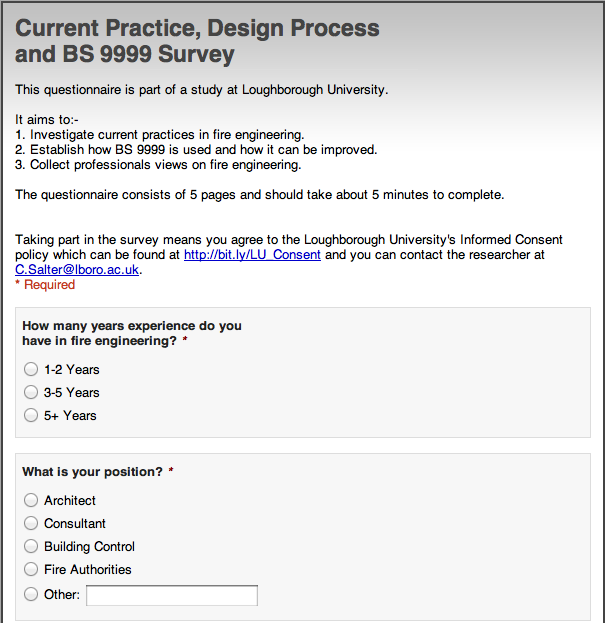
\includegraphics[width = 10 cm]{./Images/Webform}
\caption{Google Documents Webform}
\label{fig:Webform}
\end{figure}

A version of the questionnaire was also created in Microsoft Word and sent out via email. This file was protected by a password and would therefore, only allow the respondents to reply by ticking the checkboxes and writing in the given text areas. This was made as this would allow the form to be printed as well should a respondent feel that they would prefer to complete the questionnaire on paper. The Word questionnaire contained exactly the same questions as the online version and was distributed with the Loughborough University informed consent form. The Word questionnaire can be viewed in full in Appendix \ref{app:Questionnaire}.
\\
\
Questionnaires were sent to the local building authorities where it was expected that the building work present would encompass the use of BS 9999, such as the larger, more active, control authorities in larger cities. Building control offices were initially contacted to see if they would be able to fill in a questionnaire and once they responded, a questionnaire was sent out. The full list of who received the questionnaire and the outcome is shown below in Table \ref{tab:Build_Auth}. A ``no reply'' means that the initial request for the questionnaire was left unanswered. In the case of London Building Control, they felt they were in no position to answer the questionnaire. Birmingham and Leeds replied that they felt they could answer the questionnaire and one was sent to both offices. However, even after chasing up of the replies, neither managed to return the questionnaire.

\begin{table}[htbp]
	\begin{center}
	\begin{tabular}{ll}
		\toprule
		\textbf{Building Control Authority} & \textbf{Outcome of Contact} \\
		\midrule
		Birmingham	& Questionnaire Sent - No reply \\
		City of London 	& No reply \\
		Leeds	& Questionnaire Sent - No reply \\
		Leicester & Returned Completed \\
		London Building Control	& Replied - Unable to answer \\
		Manchester	& No reply \\
		Nottingham	& No reply	\\
		\bottomrule
	\end{tabular}
	\end{center}
\caption{Outcomes of Emails to Building Control}
\label{tab:Build_Auth}
\end{table}

The architects that were contacted for the questionnaire were chosen due to the large size of the firms in question. This list had already been compiled by Loughborough University from architect offices that had expressed an interest in helping research undertaken by the university. It was assumed that these larger firms would have had a greater amount of experience with larger projects where BS 9999 would potentially be more widely used. It was also assumed that the response rate would be better as there are more architects in these companies and thus multiple architects within the same firm could reply.

\begin{longtable}{ll}
\toprule
\textbf{Company} & \textbf{Outcome of Contact} \\
\midrule
\endhead

\bottomrule
\multicolumn{2}{c}{} \\
\caption{Outcomes of Emails to Architect Firms} \label{tab:architects} \\
\endfoot

ADP & Initial Email \\
Aedas & Uncontactable \\
Assael Architecture & Initial Email \\
Aukett Fitzroy Robinson & Initial Email \\
Austin-Smith:Lord & Initial Email \\
Barton Willmore & Initial Email \\
BLS (Hamiltons) & Initial Email \\
Bond Bryan Architects & Initial Email \\
BPTW Partnership & Returned \\
Broadway Malyan &Initial Email \\
Building Design Partnership Ltd & Returned \\
Carey Jones & Initial Email \\
Chetwoods & Initial Email \\
Cooper Cromar & Initial Email \\
David Wilson Partnership & Questionnaire Sent \\
DLA Architecture & Initial Email \\
DLG Architects & Initial Email \\
Donald Insall Associates & Initial Email \\
EPR Architects & Questionnaire Sent \\
Eric Parry Architects & Initial Email \\
ESA & Initial Email \\
EWA Architects & Initial Email \\
Feilden and Mawon & Initial Email\\
Fellden Clegg Bradley Studios & Initial Email \\
Fletcher Priest Architects & Initial Email \\
Foster and Partners & Initial Email \\
GHM Group & Initial Email \\
Glenn Howells & Initial Email \\
Hadfield Cawkwell Davidson & Initial Email \\
Haskoll & Returned \\
Hawkins/Brown & Initial Email \\
HKR Architects &Initial Email \\
HLM Architects & Initial Email \\
HOK & Initial Email \\
Holder Mathias Architects & Initial Email \\
Holmes Partnership & Initial Email \\
Hopkins & Initial Email \\
HTA & Initial Email \\
Hunter and Ptnrs & Initial Email \\
Ian Simpson Architects & Initial Email \\
John McAlsan and Ptnrs & Initial Email \\
John Thomspon and Ptnrs & Initial Email \\
Justico and Whiles & Initial Email \\
Levitt Bernstein Associates & Initial Email \\
Llewellyn Davies Yeang & Initial Email \\
MAKE & Returned \\
Michael Laird Architects & Initial Email \\
NBBJ & Initial Email \\
Pascall and Watson Architects & Initial Email \\
Paul Davis and Partners & Initial Email \\
Penoyre and Prasad & Initial Email \\
Pick Everard & Initial Email \\
PTE Architects & Initial Email \\
Powell Dobson & Initial Email \\
Pozzoni & Initial Email \\
PRP Architects & Returned \\
RH Partnership Architects & Replied - Cant help \\
RHWL Architects & Initial Email \\
Roger Stirk Harbour and Ptnrs & Initial Email \\
Rolfe Judd & Initial Email \\
SHCA & Questionnaire Sent \\
Sidell Gibson & Initial Email \\
SOM & Initial Email \\
Stephen George and Ptnrs & Initial Email \\
Stock Woolstencroft & Initial Email \\
Stride Treglown & Initial Email \\
Taylor Young & Initial Email \\
Wilkinson Eyre Architects & Initial Email \\

\end{longtable}



68 different architect companies were contacted as part of the questionaire. The majority didn't return the email, whilst a small minority replied stating that they were unable to help. In one case, the email sent was undelivrable and contact couldn't be made with the company.
\\
\\
With the fire engineering consultants, questionnaires were sent to various firms. The fire engineering consultants used in both the interview and questionnaire were chosen as they advertised publically via literature and websites, the fact that they undertook fire engineering work. From the writers experience, some engineering firms do not advertise fire engineering consultancy to the public and keep the consultancy ``in house''. Therefore this made it slightly harder to find consultants to answer the questionnaire.

\begin{table}[htbp]
	\begin{center}
	\begin{tabular}{ll}
		\toprule
		\textbf{Fire Consultant} & \textbf{Outcome of Contact} \\
		\midrule
		Arup	& Returned \\
		BRE	& Returned \\
		Buro Happold	& Returned \\
		Hoare Lea	& No reply \\
		Jeremy Gardner Associates	& Returned \\
		Trenton Fire	& No reply \\
		WSP	& No reply \\
		\bottomrule
	\end{tabular}
	\end{center}
		\caption{Outcomes of Emails to Fire Engineering Consultants}
		\label{tab:Fire_Consultants}
\end{table}

These consultants were asked to give the questionnaire to as many engineers within the company as possible, however, all of the companies only returned one questionnaire each.
\\
\\
As well as the email distribution method and the online survey, the questionnaire was also distributed to all delegates at the First Integrated Risk Management Planning Conference at Loughborough University on 14\textsuperscript{th} April 2010. This conference was attended by delegates from various \ac{FRS}'s, insurance companies and fire engineering consultants. All delegates received the questionnaire in the delegate pack, along with a stamped, addressed envelope to return the questionnaire if they didn't get a chance to fill it in during the conference itself. 66 delegates attended the conference.
\\
\\
The last distribution method was an placing the questionnaire in an \ac{FPA} email newsletter - a link to the online version of the questionnaire was sent out in this email to all \ac{FPA} members. It is unclear the potential audience of this newsletter as the \ac{FPA} did not share how many people this newsletter is sent to. The target audience of the \ac{FPA} email is varied with members being in a multitude of different areas relating to fire.

\subsection{Interviews}
\label{sec:Interviews}
With the small response rate from the questionnaire, more in depth detail needed to be gained. From reading the responses, it became apparent that the fire design consultants were the ones who came up as being the only ones to deal with fire engineering and therefore the decision was made to conduct in depth interviews with fire engineering consultants.
\\
\\
The interviews followed a structured approach, basing the questions on the same questions in the questionnaire sent to members. This meant that answers given in the interviews could be compared to those given in the questionnaires by other respondents. However, the benefit of the interviews is that answers could be elaborated on, rather than just the multiple choice answers in the questionnaire. This would mean that extra clarification of points and extra explanation could be gained on how the fire engineers work.
\\
\\
The interview candiadates were chosen by contacting the fire engineering firms mentioned in Table \ref{tab:Fire_Consultants}. These consultancies were contacted and asked if any engineers would be available for an interview and a time and date were arranged. In addition to the consultancies above, interviews were conducted with two consultants that were not involved in a large organisation and were involved in smaller consultancies. These were found by speaking to the other consultants and approached to see if they wished to be involved in the interview stage.


% Remove all below this line when creating thesis from Master Document
%TC:ignore
% Sets Texcount to Ignore
\appendix
\begin{singlespace}
\chapter{FDR 1 Data}
\label{app:FDR1 Data}

\lstset{caption={FDR 1 Filtering Code in Full},label=code:FDR1_Data}
\begin{lstlisting}

::Script
E:
cd "E:\Documents\IRMP Data\DATA ANALYSIS\FDR1 DATA"
sed -n 1p Lboro_9908.csv > Filtered_Buildings.csv
awk -F , "$14=="9" {print}" Lboro_9908.csv >> Filtered_Buildings.csv
awk -F , "$14=="109" {print}" Lboro_9908.csv >> Filtered_Buildings.csv
awk -F , "$14=="113" {print}" Lboro_9908.csv >> Filtered_Buildings.csv
awk -F , "$14=="121" {print}" Lboro_9908.csv >> Filtered_Buildings.csv
awk -F , "$14=="122" {print}" Lboro_9908.csv >> Filtered_Buildings.csv
awk -F , "$14=="123" {print}" Lboro_9908.csv >> Filtered_Buildings.csv
awk -F , "$14=="129" {print}" Lboro_9908.csv >> Filtered_Buildings.csv
awk -F , "$14=="131" {print}" Lboro_9908.csv >> Filtered_Buildings.csv
awk -F , "$14=="133" {print}" Lboro_9908.csv >> Filtered_Buildings.csv
awk -F , "$14=="141" {print}" Lboro_9908.csv >> Filtered_Buildings.csv
awk -F , "$14=="142" {print}" Lboro_9908.csv >> Filtered_Buildings.csv
awk -F , "$14=="144" {print}" Lboro_9908.csv >> Filtered_Buildings.csv
awk -F , "$14=="146" {print}" Lboro_9908.csv >> Filtered_Buildings.csv
awk -F , "$14=="151" {print}" Lboro_9908.csv >> Filtered_Buildings.csv
awk -F , "$14=="152" {print}" Lboro_9908.csv >> Filtered_Buildings.csv
awk -F , "$14=="161" {print}" Lboro_9908.csv >> Filtered_Buildings.csv
awk -F , "$14=="162" {print}" Lboro_9908.csv >> Filtered_Buildings.csv
awk -F , "$14=="163" {print}" Lboro_9908.csv >> Filtered_Buildings.csv
awk -F , "$14=="174" {print}" Lboro_9908.csv >> Filtered_Buildings.csv
awk -F , "$14=="175" {print}" Lboro_9908.csv >> Filtered_Buildings.csv
awk -F , "$14=="176" {print}" Lboro_9908.csv >> Filtered_Buildings.csv
awk -F , "$14=="178" {print}" Lboro_9908.csv >> Filtered_Buildings.csv
awk -F , "$14=="179" {print}" Lboro_9908.csv >> Filtered_Buildings.csv
awk -F , "$14=="181" {print}" Lboro_9908.csv >> Filtered_Buildings.csv
awk -F , "$14=="182" {print}" Lboro_9908.csv >> Filtered_Buildings.csv
awk -F , "$14=="183" {print}" Lboro_9908.csv >> Filtered_Buildings.csv
awk -F , "$14=="185" {print}" Lboro_9908.csv >> Filtered_Buildings.csv
awk -F , "$14=="186" {print}" Lboro_9908.csv >> Filtered_Buildings.csv
awk -F , "$14=="189" {print}" Lboro_9908.csv >> Filtered_Buildings.csv
awk -F , "$14=="219" {print}" Lboro_9908.csv >> Filtered_Buildings.csv
awk -F , "$14=="249" {print}" Lboro_9908.csv >> Filtered_Buildings.csv
awk -F , "$14=="261" {print}" Lboro_9908.csv >> Filtered_Buildings.csv
awk -F , "$14=="309" {print}" Lboro_9908.csv >> Filtered_Buildings.csv
awk -F , "$14=="311" {print}" Lboro_9908.csv >> Filtered_Buildings.csv
awk -F , "$14=="322" {print}" Lboro_9908.csv >> Filtered_Buildings.csv
awk -F , "$14=="331" {print}" Lboro_9908.csv >> Filtered_Buildings.csv
awk -F , "$14=="332" {print}" Lboro_9908.csv >> Filtered_Buildings.csv
awk -F , "$14=="341" {print}" Lboro_9908.csv >> Filtered_Buildings.csv
awk -F , "$14=="345" {print}" Lboro_9908.csv >> Filtered_Buildings.csv
awk -F , "$14=="359" {print}" Lboro_9908.csv >> Filtered_Buildings.csv
awk -F , "$14=="369" {print}" Lboro_9908.csv >> Filtered_Buildings.csv
awk -F , "$14=="409" {print}" Lboro_9908.csv >> Filtered_Buildings.csv
awk -F , "$14=="449" {print}" Lboro_9908.csv >> Filtered_Buildings.csv
awk -F , "$14=="469" {print}" Lboro_9908.csv >> Filtered_Buildings.csv
awk -F , "$14=="489" {print}" Lboro_9908.csv >> Filtered_Buildings.csv
awk -F , "$14=="509" {print}" Lboro_9908.csv >> Filtered_Buildings.csv
awk -F , "$14=="511" {print}" Lboro_9908.csv >> Filtered_Buildings.csv
awk -F , "$14=="581" {print}" Lboro_9908.csv >> Filtered_Buildings.csv
awk -F , "$14=="585" {print}" Lboro_9908.csv >> Filtered_Buildings.csv
awk -F , "$14=="591" {print}" Lboro_9908.csv >> Filtered_Buildings.csv
awk -F , "$14=="593" {print}" Lboro_9908.csv >> Filtered_Buildings.csv
awk -F , "$14=="597" {print}" Lboro_9908.csv >> Filtered_Buildings.csv
awk -F , "$14=="659" {print}" Lboro_9908.csv >> Filtered_Buildings.csv
awk -F , "$14=="700" {print}" Lboro_9908.csv >> Filtered_Buildings.csv
awk -F , "$14=="815" {print}" Lboro_9908.csv >> Filtered_Buildings.csv
awk -F , "$14=="881" {print}" Lboro_9908.csv >> Filtered_Buildings.csv
awk -F , "$14=="882" {print}" Lboro_9908.csv >> Filtered_Buildings.csv
awk -F , "$14=="888" {print}" Lboro_9908.csv >> Filtered_Buildings.csv
awk -F , "$14=="891" {print}" Lboro_9908.csv >> Filtered_Buildings.csv
awk -F , "$14=="900" {print}" Lboro_9908.csv >> Filtered_Buildings.csv
awk -F , "$14=="901" {print}" Lboro_9908.csv >> Filtered_Buildings.csv
awk -F , "$14=="904" {print}" Lboro_9908.csv >> Filtered_Buildings.csv
awk -F , "$14=="909" {print}" Lboro_9908.csv >> Filtered_Buildings.csv
awk -F , "$14=="926" {print}" Lboro_9908.csv >> Filtered_Buildings.csv
awk -F , "$14=="953" {print}" Lboro_9908.csv >> Filtered_Buildings.csv
awk -F , "$14=="959" {print}" Lboro_9908.csv >> Filtered_Buildings.csv
\end{lstlisting}

\newpage

\begin{longtable}{|l|p{11cm}|}

\caption{FDR 1 TOP Codes and Descriptions} \label{tab:TOP_Codes} \\
\hline
\textbf{FDR 1 Code}	& \textbf{FDR1 Description}\\
\hline
\endhead

\hline
\endfoot
\rowcolor{lightgray} 9	&Public administration and defence building other than elsewhere. codable e.g. office	\\
109	&Other building for public assembly, entertainment, recreation etc (not elsewhere specified, Sports and social club)	\\
\rowcolor{lightgray} 113	&Amusement Arcades	\\
121	&Dance Halls	\\
\rowcolor{lightgray} 122	&Exhibition Halls	\\
123	&Sports Stadia	\\
\rowcolor{lightgray} 129	&Other Sports Facilities\\
131	&Building Of Worship	\\
\rowcolor{lightgray} 133	&Church Halls	\\
141	&Social Clubs	\\
\rowcolor{lightgray} 142	&Sports Clubs, Clubs for Recreational and Other Cultural Entertainment	\\
144	&Casino	\\
\rowcolor{lightgray} 146	&Youth Clubs	\\
151	&Libraries	\\
\rowcolor{lightgray} 152	&Museums, Art Galleries	\\
161	&Restaurant (Cafes Take Away Food Shops)\\
\rowcolor{lightgray} 162	&Night-Clubs	\\
163	&Public Houses	\\
\rowcolor{lightgray} 174	&Railway Station Building, surface	\\
175	&Railway Station Building, sub-surface	\\
\rowcolor{lightgray} 176	&Railway Station Building, above surface\\
178	&Railway Station Building, unspecified	\\
\rowcolor{lightgray} 179	&Passenger terminal	\\
181	&Theatre	\\
\rowcolor{lightgray} 182	&Concert Hall	\\
183	&Cinema	\\
\rowcolor{lightgray} 185	&Radio/TV Studio	\\
186	&Film Studio	\\
\rowcolor{lightgray} 189	&Other Theatres/Studios	\\
219	&Schools Etc	\\
\rowcolor{lightgray} 249	&Further Education Establishment (Non Residential)	\\
261	&Conference Centres	\\
\rowcolor{lightgray} 309	&Other type of welfare or charitable establishment	\\
311	&Old Persons Rest Home	\\
\rowcolor{lightgray} 322	&Children's Home	\\
331	&Hospital - Psychiatric Or Mentally Handicapped	\\
\rowcolor{lightgray} 332	&Hospital - Other	\\
341	&Prison and Remand Centres	\\
\rowcolor{lightgray} 345	&Police Stations	\\
359	&Home for physically handicapped or disabled (other than children)	\\
\rowcolor{lightgray} 369	&Home for mentally handicapped or disabled (other than children)	\\
409	&Other establishment providing accommodation (excluding penal Establishments)	\\
\rowcolor{lightgray} 449	&Hotel, Boarding House or Guest Hose	\\
469	&Block accommodation for occupational, religious, national etc groups	\\
\rowcolor{lightgray} 489	&Establishment providing short-stay accommodation for recreational purposes	\\
509	&Single Shop	\\
\rowcolor{lightgray} 511	&Supermarket	\\
581	&Department Store	\\
\rowcolor{lightgray} 585	&Shopping Mall/Centre/Indoor Market	\\
591	&Offices - permanent stand alone structure	\\
\rowcolor{lightgray} 593	&Other Medical or Dental Establishments	\\
597	&Offices - Temporary	\\
\rowcolor{lightgray} 659	&Agricultural buildings	\\
700	&Industrial Premises	\\
\rowcolor{lightgray} 815	&Zoo	\\
881	&Private garage	\\
\rowcolor{lightgray} 882	&Car Park Building (Separate From Other Building)\\
888	&Fire stations	\\
\rowcolor{lightgray} 891	&Warehouse	\\
900	&Building, not specified	\\
\rowcolor{lightgray} 901	&Public Lavatories	\\
904	&Other private non-residential building	\\
\rowcolor{lightgray} 909	&Building, miscellaneous	\\
926	&Private shed or greenhouse	\\
\rowcolor{lightgray} 953	&Railway, without building	\\
959	&Railway, building other than station\\
\end{longtable}

\chapter{Questionnaire}
\label{app:Questionnaire}

\section{Pilot Study}
\label{app:Pilot Study}
\textbf{Personal Questions}
\begin{enumerate}
\item How many years have you spent in the fire engineering trade?
\item What is your relation to the fire engineering trade?
\end{enumerate}

\textbf{Design Phase}
\begin{enumerate}
\item Do you spend time risk assessing the property?
\item If you do a risk assessment, how do you carry out or identify the hazards?
\item At what stage are you normally brought onto the project?
\item When is a more suitable time to be brought onto the project?
\item Do you believe that not being brought onto a project early can affect the costs of the final project?
\item Do your designs only focus on life safety?
\item Are the majority of your designs mainly code compliant with a few ``trade offs'' for non code compliant areas?
\item Do you build in any form of redundancy into your designs?
\item Would you say your designs are inherently safe?
\end{enumerate}

\textbf{Costs}
\begin{enumerate}
\item In your design decisions, is cost the critical design factor?
\item Do you consider the costs of protection measures you specify?
\end{enumerate}

\textbf{Fire Protection}
\begin{enumerate}
\item Do you have to validate/verify your non code compliant designs?
\item Is there any guidance on what should be validated or verified?
\item How do you prove that a design you are proposing is equivalent to that specified in the codes?
\item How does the approvals process work?
\item Do you believe that Building Control reject your plans due to a lack of understanding in Fire Engineering?
\item Buildings are relying more on good design and less on active systems for ventilation and the like. Can you see fire engineering following this trend?
\item Do you specify extra passive fire protection rather than that just described in the codes?
\item If a certain protection method lowered costs for insurance for a building, would you specifiy that protection measure?
\item On a scale of 1-5, how essential do you think passive fire protection is?
\item On a scale of 1-5, how effective do you think passive fire protection is?
\end{enumerate}

\textbf{BS 9999}
\begin{enumerate}
\item How often do you use BS 9999 over other current codes?
\item Has BS 9999 changed your methods of design work?
\item Part of BS 9999 focuses on building management and the management of the building after completion. Do you provide the management plans?
\item Do you believe that BS 9999 reduces the scope for fire engineering?
\item Do you believe that BS 9999 offers a more cost effective method of design?
\item Does a design using BS 9999 take less time to complete a design, on average, than with previous design codes?
\item How have other project stakeholders taken to BS9999?
\item Do you believe that BS 9999 will help building owners comply with The Regulatory Reform Order?
\item Do you believe that the addition of sprinklers to reduce a risk profile is cost effective?
\item Do you still design non code compliant areas within buildings?
\item Do you think BS 9999 will have a positive effect on the management of the building's passive fire protection measures?
\item Considering the building is tailored to a specific risk profile, how severe can you see a change of risk profile being in the future?
\end{enumerate}


\newpage
\section{Questionnaire}
\label{app:Questionnaire}
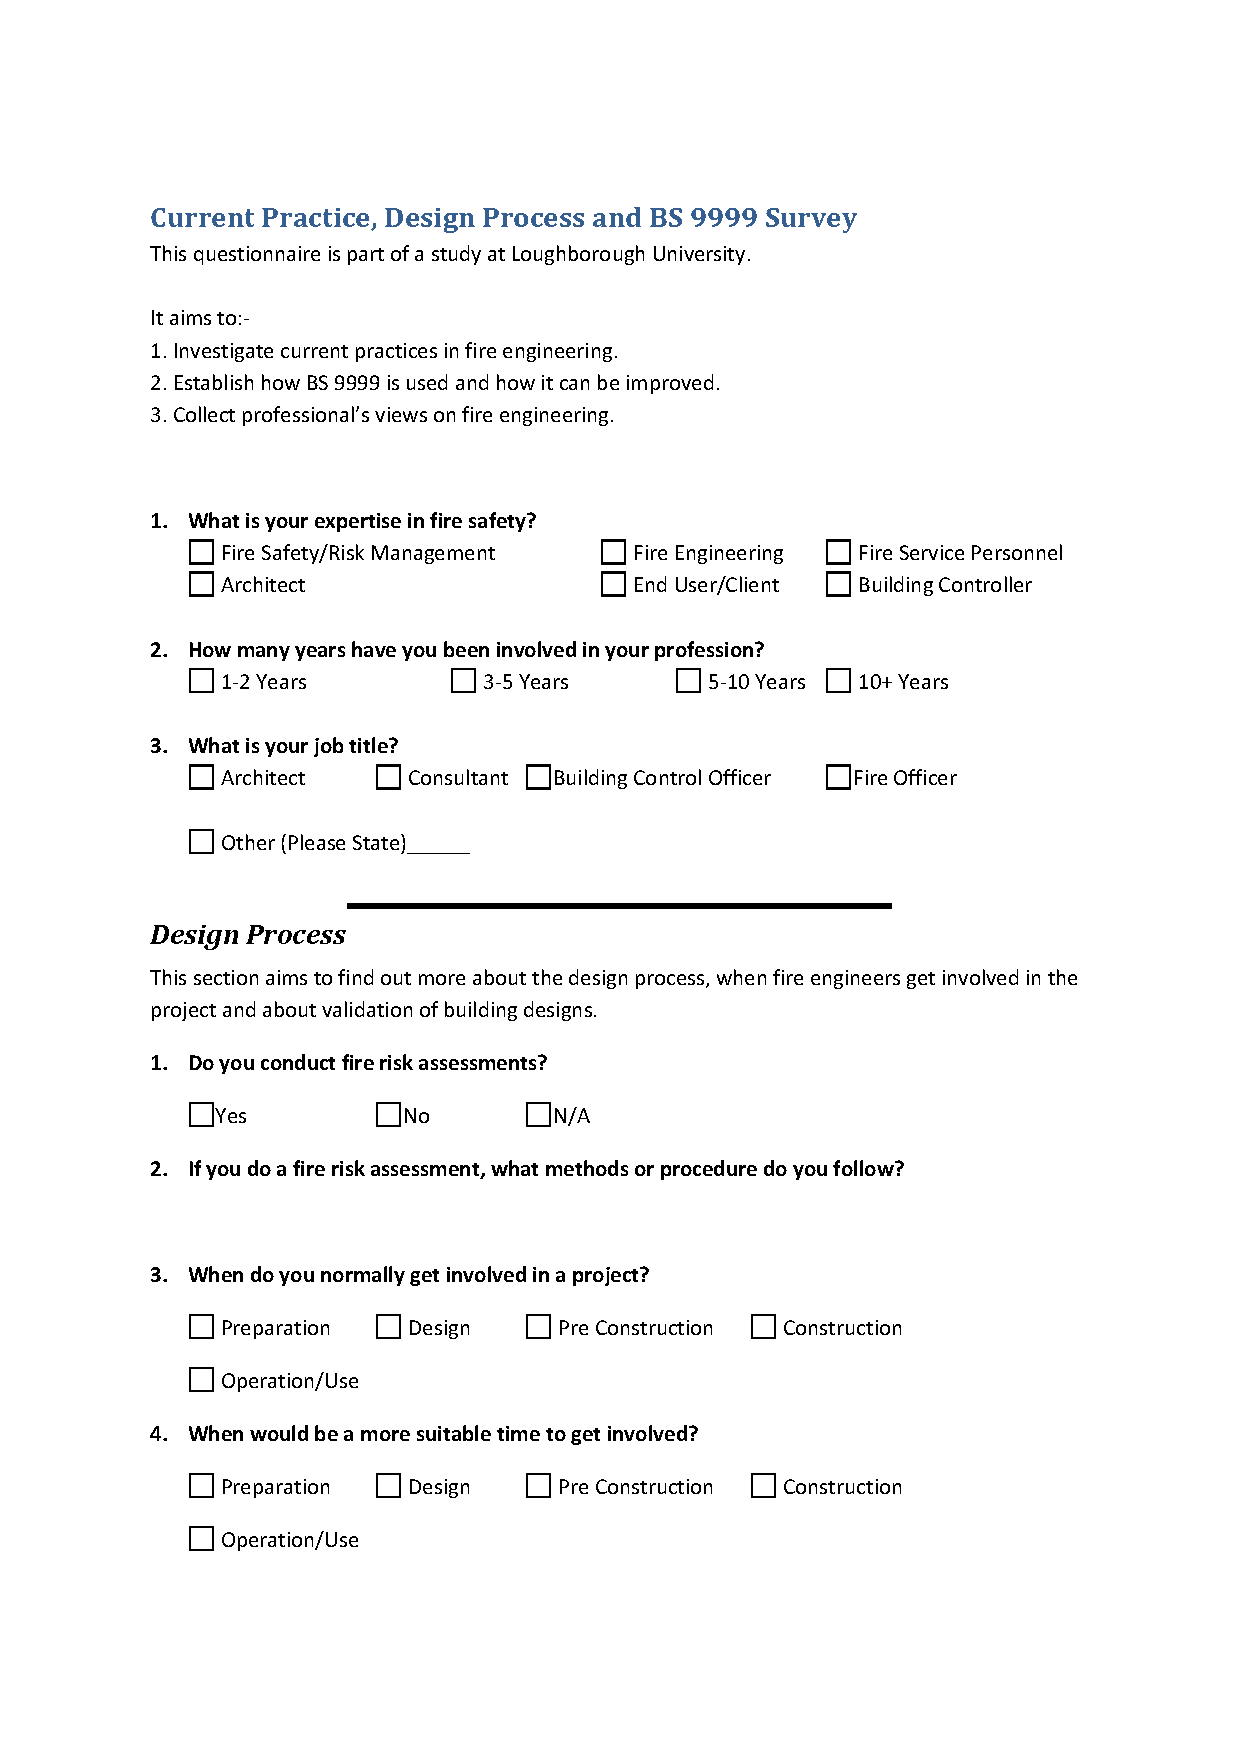
\includepdf[pages=1-,pagecommand={\thispagestyle{fancy}}]{10-04-16_Generic_Questionnaire_Online}

\addcontentsline{toc}{section}{Bibliography}
\bibliographystyle{custom}
\bibliography{../../../Bibliography}

\end{singlespace}
\end{document}